% Chapter 5

\chapter{Experimental results} % Main chapter title

\label{Chapter5} % For referencing the chapter elsewhere, use \ref{Chapter5} 

%----------------------------------------------------------------------------------------
\section{Introduction}
In the previous chapters we described how the DeepMiRNA's architecture is based on two main functional blocks: on one side there is the NN, whose purpose is that of analyzing the selected candidate target sites, while on the other there are the CSSM used during the target prediction step and the a-posteriori filter that tries to refine the network prediction. 

To assess these two aspects, we first evaluated the outputs of the NN training process through cross validation and then investigated performance using the different candidate site selection methods outlined in chapter \ref{Chapter3}. These comprised the novel (non-canonical) models implemented for this thesis: CSS-6.10 and CSS-7.10. Finally, we tested DeepMiRNA’s performance by comparing it against TargetScan\cite{targetscan}, mirDB\cite{mirdb} and miRAW\cite{miraw}, which represent the most commonly used target site predictors based on citations.

The experimental results present in this chapter concern the best pipeline configuration for DeepMiRNA. This comprises the use of the feed-forward neural network that exhibited an overall better performance than the convolutional model, especially in the identification of negative binding sites. 

There can be many reason explaining this differences, but we believe that the lack of a consistent dataset of negatively validated binding sites may be the principal cause. 

\section{Neural Netework evaluation}
The best performing feed-forward neural network was trained using the whole training set with this parameters:

\begin{itemize}
	\item dropout rate = 0.7
	\item optimizer = Adam as described in chapter \ref{Chapter4}
	\item loss function = binary cross entropy
	\item batch size = 128
	\item number of epochs = 15
\end{itemize}

The above parameters where computed using a validation set composed of about 10000 examples (20\% of the training set).

Once the best model has been selected, we built a fresh network using the best parameters and we trained it holding out the 25\% of the training data for the purpose of testing its performance. This validation presented very good results in terms of predicting both positive and negative sites, with all evaluated metrics resulting in scores well above 0.9 (see figure\ref{fig:network_evaluation}).

\begin{figure}[hbt!]
	\centering
	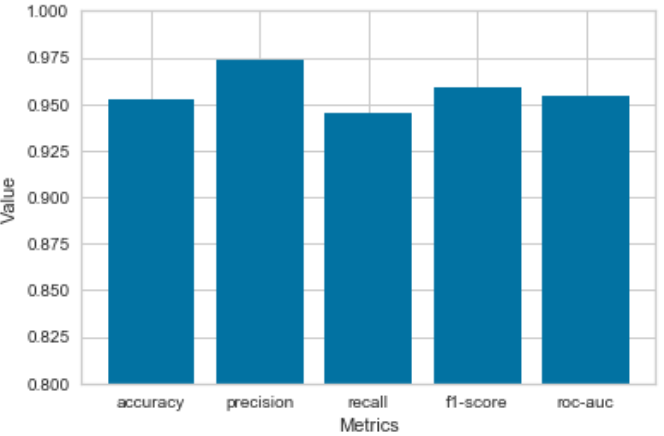
\includegraphics[width=\textwidth]{Figures/network_evaluation}
	\caption{\textbf{Network performance metrics.} To this purpose we trained the network with best parameters using 75\% of the training data. The remaining 25\% has been used as test set. As shown above all metrics are close to 0.95.}
	\label{fig:network_evaluation}
\end{figure}

\section{The role of the candidate site selection method}
To investigate the impact of the site selection method, we compared the performances of the three different CSSM described in chapter\ref{Chapter3}. 

Figure \ref{fig:cssm} summaries the obtained results: all methods reach accuracies between 0.8 and 0.82, these values are computed considering the imbalance of the test set, that is they are calculated as the average of the accuracies on positive and negative samples. CSS-6.0:10 seems to achieve slightly better performances for every metric but precision, compared to the other two methods. The F1-score is the harmonic average between precision and recall and shows how well both classes are classified by a particular CSSM. The values obtained are very similar to the accuracies and indicate an ability to effectively predict both negative and positive targets especially for CSS-6.0:10 and CSS-7.0:10.

\begin{figure}[hbt!]
	\centering
	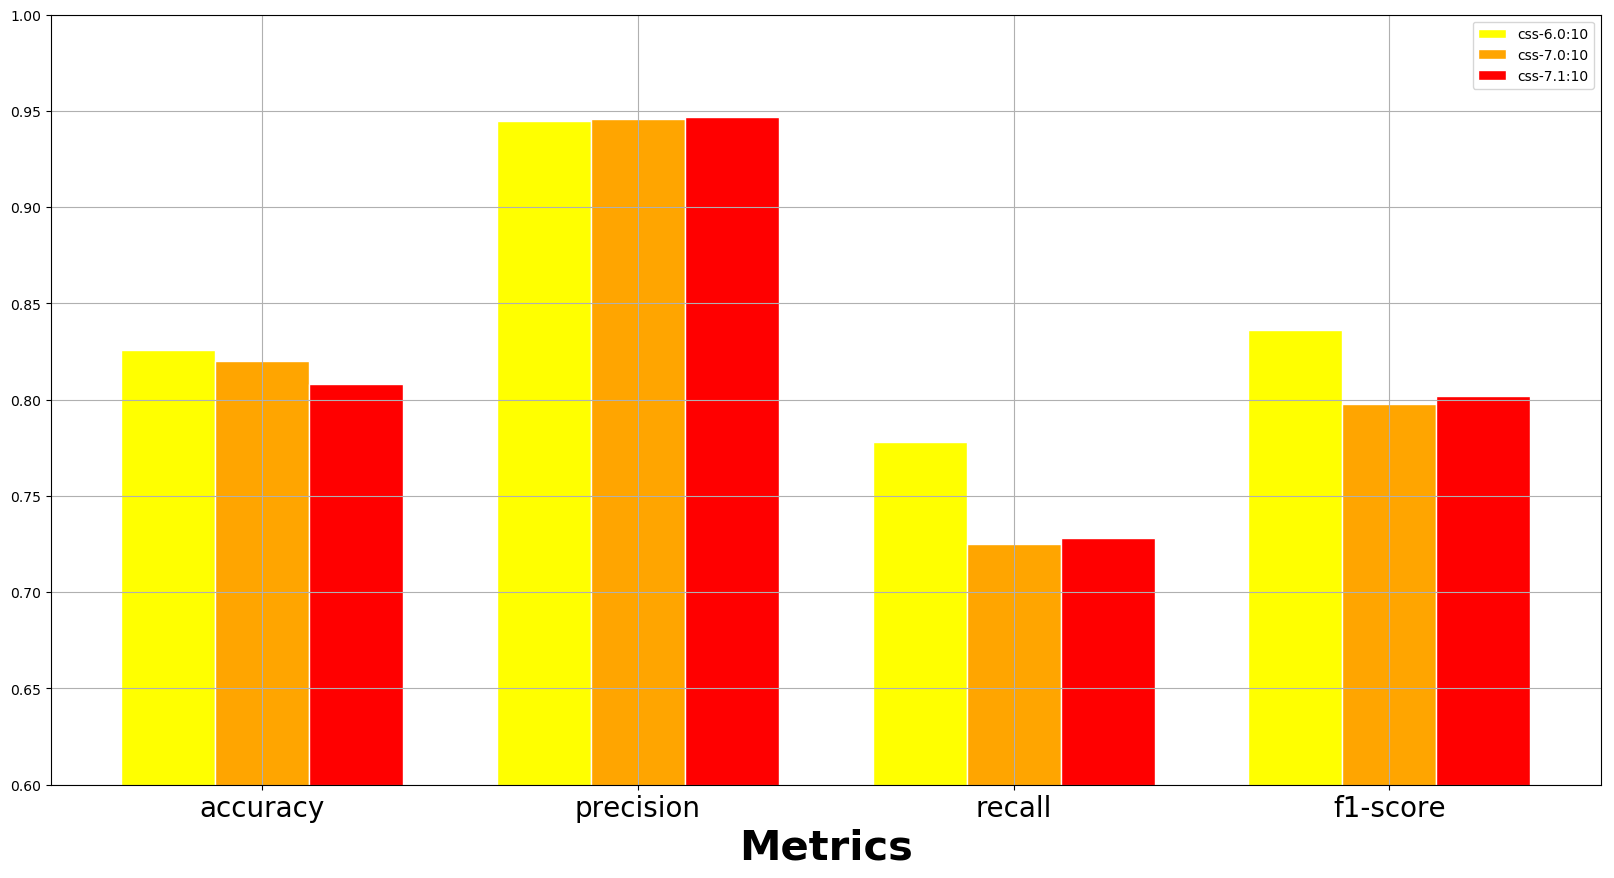
\includegraphics[width=\textwidth]{Figures/cssm_evaluation}
	\caption{\textbf{Evaluation of DeepMiRNA different candidate site selection methods.} Results are evaluated in terms of balanced accuracy, precision, recall and f1-score. The best result was achieved using CSS-6.0:10.}
	\label{fig:cssm}
\end{figure}

\section{Site accessibility filter}
In order to measure the effect of site accessibility on miRNA target prediction, we tested the best performing pipeline configuration without filtering the network output. While this reduces the computational cost of the whole process, DeepMiRNA becomes slightly more biased towards the prediction of positive sites. However, this is true only for the convolutional model. To underline this difference we report the results obtained with both network models.

\begin{table}
	\caption{\textbf{Results with or without the a-posteriori filtering in the feed-forward network.}}
	\label{tab:ff_sa_filter}
	\centering
	\begin{tabular}{| c | c | c | c | c | c | c | c |} \hline
		\multicolumn{2}{|c|}{\textbf{Accuracies}} & \multicolumn{2}{c|}{\textbf{Precision}} & \multicolumn{2}{c|}{\textbf{Recall}} & \multicolumn{2}{c|}{\textbf{F1-score}} \\ \hline 
		\emph{NF} & \emph{WF} & \emph{NF} & \emph{WF} & \emph{NF} & \emph{WF} & \emph{NF} & \emph{WF} \\ \hline
		\textbf{0.827} & 0.82 & 0.936 & \textbf{0.939} & \textbf{0.794} & 0.785 & \textbf{0.840} & 0.838 \\ \hline
		
	\end{tabular}
\end{table}

Table \ref{tab:ff_sa_filter} shows that using a site accessibility filter (WF) with the feed-forward neural network does not improve the prediction performance, in fact, a no filter (NF) configuration actually achieves better results. This means that the rate of false negatives generated by the filter is higher than the gain derived from the reduction of the false positives. Achieving high precision means that when the network output a $1$ is almost never fails, while high values of recall implies the number of false negative is low. These results show that the feed-forward network is very precise in identifying negative binding sites, while it behaves worse with positive targets.  

For the CNN, instead, the filtering steps improves the network ability to predict miRNA's targets correctly. Table \ref{tab:cnn_sa_filter} indicates that precision, which is the fraction of all positive predictions that are actually positive, and balanced accuracies increase, while recall, that is the ability of correctly recognizing positive entries, decreases much slower. 

\begin{table}[hb!]
	\caption{\textbf{Results with or without the a-posteriori filter in the convolutional network.}}
	\label{tab:cnn_sa_filter}
	\centering
	\begin{tabular}{| c | c | c | c | c | c | c | c |} \hline
		\multicolumn{2}{|c|}{\textbf{Accuracies}} & \multicolumn{2}{c|}{\textbf{Precision}} & \multicolumn{2}{c|}{\textbf{Recall}} & \multicolumn{2}{c|}{\textbf{F1-score}} \\ \hline 
		\emph{NF} & \emph{WF} & \emph{NF} & \emph{WF} & \emph{NF} & \emph{WF} & \emph{NF} & \emph{WF} \\ \hline
		0.628 & \textbf{0.652} & 0.649 & \textbf{0.761} & \textbf{0.662} & 0.621 & 0.64 & \textbf{0.681} \\ \hline
		
	\end{tabular}
\end{table}

\section{Comparison with other miRNA target prediction tools}
Figure \ref{Chapter1} compares the performance of DeepMiRNA best configuration, that is CSS-6.0:10 without filter, with state-of-art target prediction software tools TargetScan, mirDB and miRAW using the test set defined in chapter \ref{Chapter3} 